\begin{figure}[h!]
    \begin{center}
    \caption{Effects on Public Health Spending per capita}\label{fig:9}
    \begin{subfigure}{0.48\textwidth}
        \caption{\scriptsize Health and Sanitation (Finbra)}\label{fig:9a}
        \centering
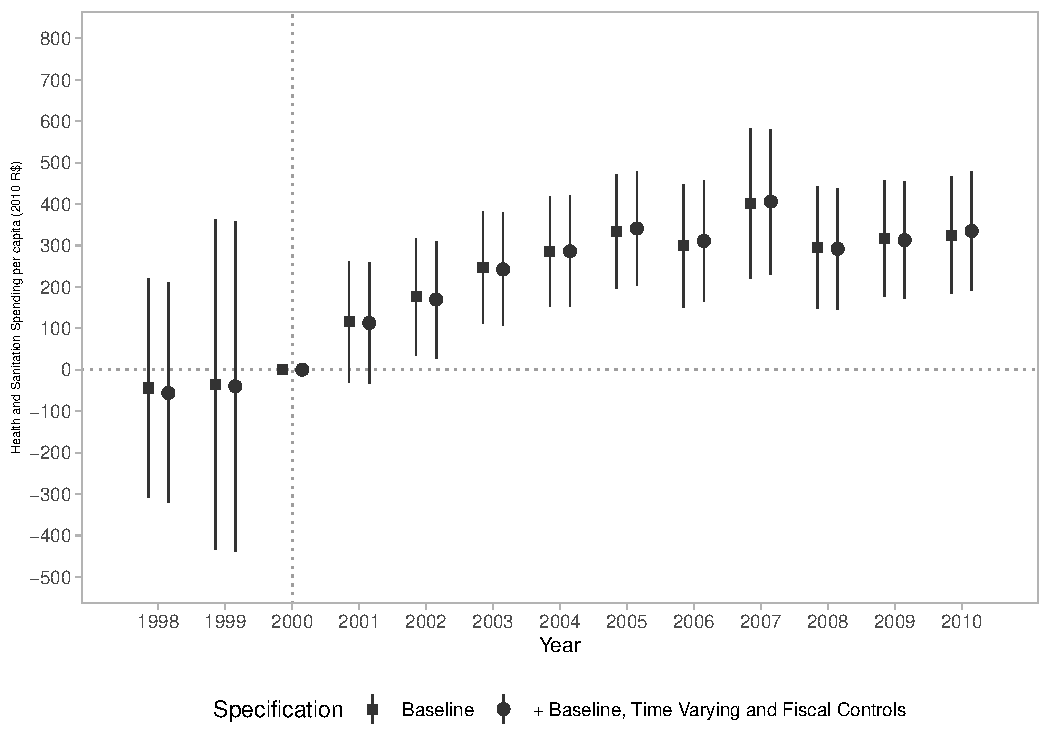
\includegraphics[width=\textwidth]{plots/finbra_desp_saude_san_pcapita_dist_ec29_baseline_dist_ec29_baseline_9.pdf}
    \end{subfigure}
    \begin{subfigure}{0.48\textwidth}
        \centering
        \caption{\scriptsize Total Health Spending (SIOPS)}\label{fig:9b}
        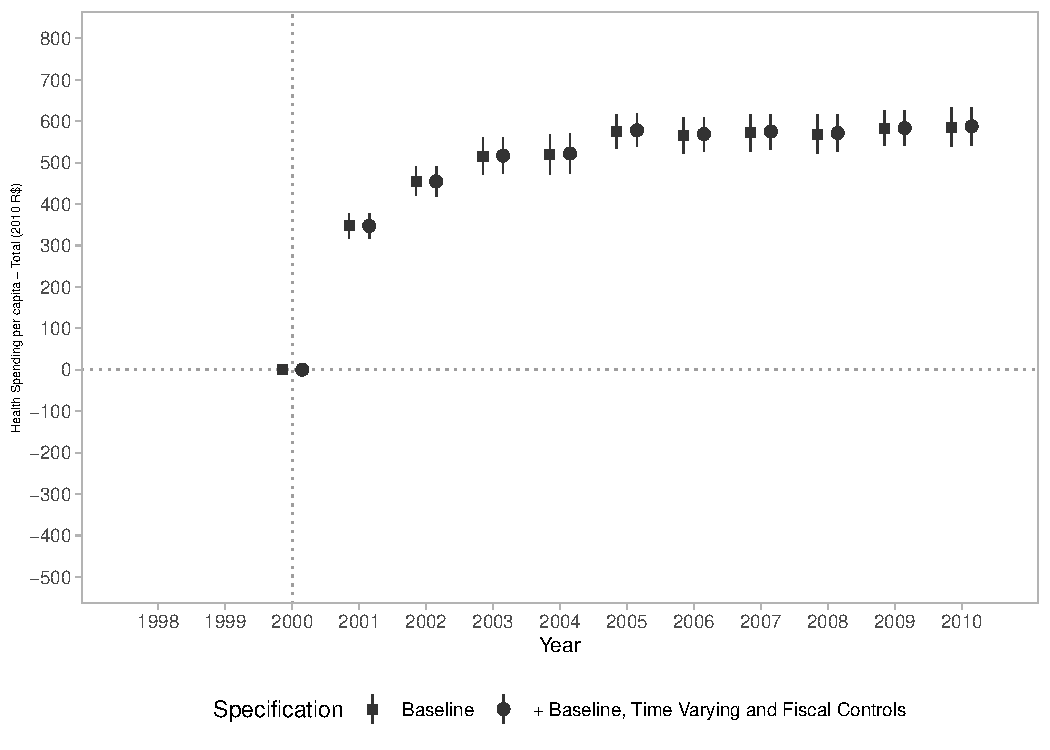
\includegraphics[width=\textwidth]{plots/siops_despsaude_pcapita_dist_ec29_baseline_dist_ec29_baseline_9.pdf}
    \end{subfigure}
    \begin{subfigure}{0.48\textwidth}
        \centering
        \caption{\scriptsize Health Spending - Own Resources (SIOPS)}\label{fig:9c}
        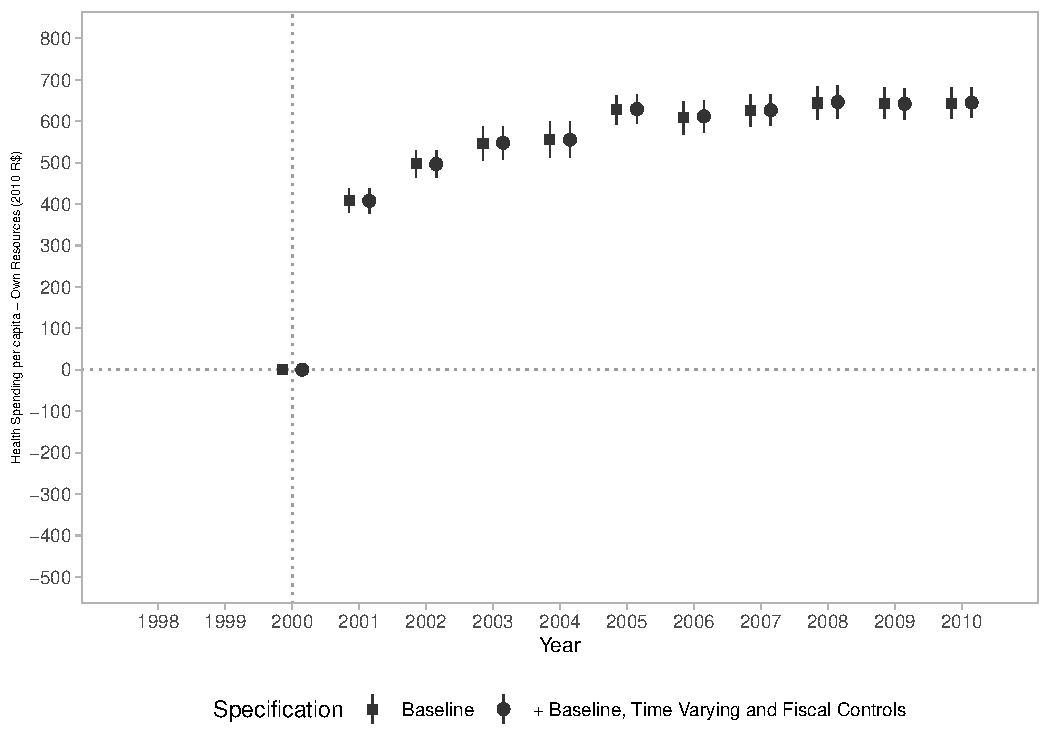
\includegraphics[width=\textwidth]{plots/siops_desprecpropriosaude_pcapita_dist_ec29_baseline_dist_ec29_baseline_9.pdf}
    \end{subfigure}
    \begin{subfigure}{0.48\textwidth}
        \centering
        \caption{\scriptsize Health Spending  - Transfers (SIOPS)}\label{fig:9d}
        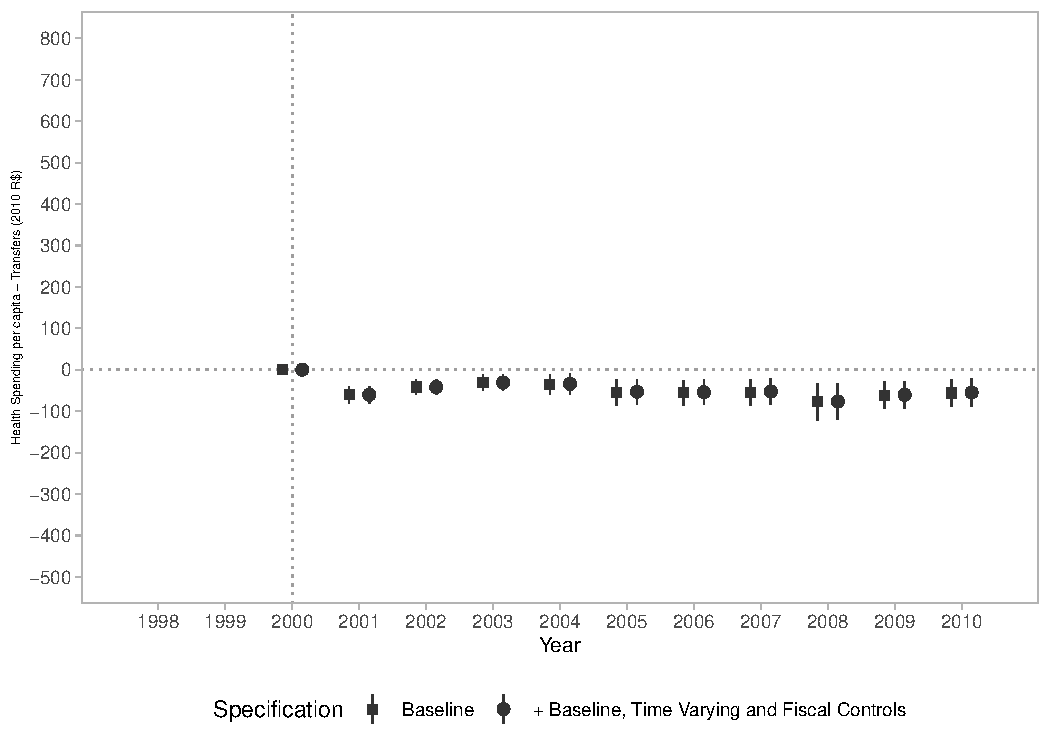
\includegraphics[width=\textwidth]{plots/siops_despexrecproprio_pcapita_dist_ec29_baseline_dist_ec29_baseline_9.pdf}
    \end{subfigure}
    
    \end{center}
    \scriptsize{Notes: The number of observations is 64224 for Figure \ref{fig:9a} and 56012 for the remaining. DiD Estimates from Equation \ref{eq:2}. Independent variable is the distance to the EC/29 target in p.p. Square dots represent the baseline model with municipality and state-year fixed effects. Round dots represent fully saturated specification (Column 4 in regression Tables). Lines represent 95\% confidence intervals. Arrows, when present, indicate confidence intervals out of the plot bounds. Standard errors are clustered in the municipality level.}
    
\end{figure}